\section{Corpus Audit and Cross-Crop Shift}
\label{sec:data}

The source corpus contains 418 high-resolution UAV RGB images: 297 Magnolia
and 121 Azalea.  Magnolia frames are $5184\!\times\!3888$ pixels and Azalea
frames are $5280\!\times\!3956$ pixels.  We retain 29,842 valid one-class plant
boxes (15,644 Magnolia; 14,198 Azalea).  Five zero-width rows are rejected by
the parser without modifying the source labels.  Three empty Azalea label
files are retained as source-level negatives, while one unmatched RGB image is
excluded.  No box extends outside its source frame, and the duplicate-image
audit finds no candidate duplicate pair.  \Cref{tab:corpus} summarizes the
frozen source, annotation, split, and tile counts.

\begin{table}[t]
\centering
\caption{Frozen corpus and source-safe split.  Tile counts include positive
and hard-negative tiles generated after the source-image split.}
\label{tab:corpus}
\small
\setlength{\tabcolsep}{3.5pt}
\begin{tabular}{lrrrr}
\toprule
Crop & Sources & Boxes & Train/Val/Test & Tiles \\
\midrule
Azalea   & 121 & 14,198 & 81/20/20  & 4,235 \\
Magnolia & 297 & 15,644 & 221/38/38 & 10,395 \\
\midrule
Total    & 418 & 29,842 & 302/58/58 & 14,630 \\
\bottomrule
\end{tabular}
\end{table}

The two crops impose a meaningful visual shift.  Azalea sources contain a
median of 97 boxes, compared with 57 for Magnolia, while the median normalized
Azalea box area is $0.00466$, 44.1\% smaller than Magnolia's $0.00833$.
Median brightness is similar (0.400 versus 0.395), but the green-pixel fraction
is lower for Azalea (0.312 versus 0.429).  These differences jointly change
object scale, density, texture, and background composition; they motivate
bidirectional transfer rather than a pooled-only report.
\begin{figure*}[t]
\centering
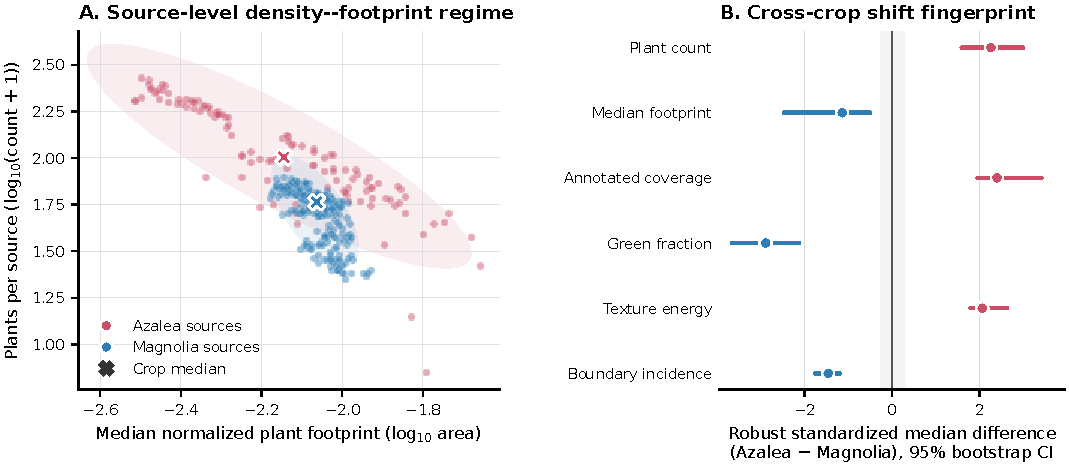
\includegraphics[width=.98\textwidth]{figures/cross_crop_signature.pdf}
\caption{Source-level cross-crop shift.  \textbf{A:} Each point is one source
image; crosses and ellipses show crop medians and 90\% covariance regions in
the density--footprint plane.  \textbf{B:} Robust standardized Azalea-minus-
Magnolia median differences with 95\% source-bootstrap confidence intervals
(1,000 resamples).  Positive values indicate larger Azalea statistics.  The
joint reversal in plant density, footprint, green fraction, and texture makes
cross-crop transfer a multivariate shift rather than a class-count imbalance.}
\label{fig:cross-crop-signature}
\end{figure*}

Across both crops, 28.96\% of boxes are close to a source-image boundary.
This is relevant because overlapping crops can preserve a box in more than one
tile; consequently, tile-level random splitting would leak near-identical
content across partitions.  We therefore use source identity as the indivisible
unit for splitting, resampling, and uncertainty estimation.
\Cref{fig:cross-crop-signature} visualizes this source-level shift without
treating correlated tiles as independent observations.
